
%---------------------------------------------------------------------------
\documentclass%%
%---------------------------------------------------------------------------
  [fontsize=11pt,%%          Schriftgroesse
%---------------------------------------------------------------------------
% Satzspiegel
   paper=a4,%%               Papierformat
   %enlargefirstpage=on,%%    Erste Seite anders
   %pagenumber=headright,%%   Seitenzahl oben mittig  
%---------------------------------------------------------------------------
% Layout
   headsepline=off,%%         Linie unter der Seitenzahl
   parskip=half,%%           Abstand zwischen Absaetzen
%---------------------------------------------------------------------------
% Was kommt in den Briefkopf und in die Anschrift
   fromalign=right,%%        Plazierung des Briefkopfs
   fromphone=off,%%           Telefonnummer im Absender
   fromlogo=on,%%            Firmenlogo
   fromrule=aftername,%%     Linie im Absender (aftername, afteraddress)
   fromfax=off,%%            Faxnummer
   fromemail=on,%%           Emailadresse
   fromurl=on, %%            Homepage
   addrfield=on,%%           Adressfeld fuer Fensterkuverts
   backaddress=on,%%         ...und Absender im Fenster
   subject=beforeopening,%%  Plazierung der Betreffzeile
   locfield=narrow,%%        zusaetzliches Feld fuer Absender
   foldmarks=on,%%           Faltmarken setzen
   numericaldate=off,%%      Datum numerisch ausgeben
   refline=narrow,%%         Geschaeftszeile im Satzspiegel
   firstfoot=off,%%           Footerbereich
%---------------------------------------------------------------------------
% Formatierung
   draft=off%%                Entwurfsmodus
]{scrlttr2}
%---------------------------------------------------------------------------
\usepackage[english, ngerman]{babel}  
\usepackage{url}
\usepackage{lmodern}
\usepackage[utf8]{inputenc} 
\usepackage{tabularx}
\usepackage{colortbl}
\usepackage{graphicx}
\usepackage{fontawesome}
% symbols: (cell)phone, email
\RequirePackage{marvosym} % for gray color in header
%\RequirePackage{color} % for gray color in header
\usepackage[T1]{fontenc}
%---------------------------------------------------------------------------
% Schriften werden hier definiert
\renewcommand*\familydefault{\sfdefault} % Latin Modern Sans
\setkomafont{fromname}{\sffamily\color{mygray}\LARGE}
%\setkomafont{pagenumber}{\sffamily}
\setkomafont{subject}{\mdseries}
\setkomafont{backaddress}{\mdseries}
\setkomafont{fromaddress}{\small\sffamily\mdseries\color{mygray}}
%---------------------------------------------------------------------------
\begin{document}
%---------------------------------------------------------------------------
% Briefstil und Position des Briefkopfs
\LoadLetterOption{DIN} %% oder: DINmtext, SN, SNleft, KOMAold.
\makeatletter
\@setplength{sigbeforevskip}{17mm} % Abstand der Signatur von dem closing
\@setplength{firstheadvpos}{17mm} % Abstand des Absenderfeldes vom Top
\@setplength{firstfootvpos}{275mm} % Abstand des Footers von oben
\@setplength{firstheadwidth}{\paperwidth}
\@setplength{locwidth}{70mm}   % Breite des Locationfeldes
\@setplength{locvpos}{65mm}    % Abstand des Locationfeldes von oben
\ifdim \useplength{toaddrhpos}>\z@
  \@addtoplength[-2]{firstheadwidth}{\useplength{toaddrhpos}}
\else
  \@addtoplength[2]{firstheadwidth}{\useplength{toaddrhpos}}
\fi
\@setplength{foldmarkhpos}{6.5mm}
\makeatother
%---------------------------------------------------------------------------
% Farben werden hier definiert
% define gray for header
\definecolor{mygray}{gray}{.55}
% define blue for address
\definecolor{myblue}{rgb}{0.25,0.45,0.75}

%---------------------------------------------------------------------------
% Absender Daten
%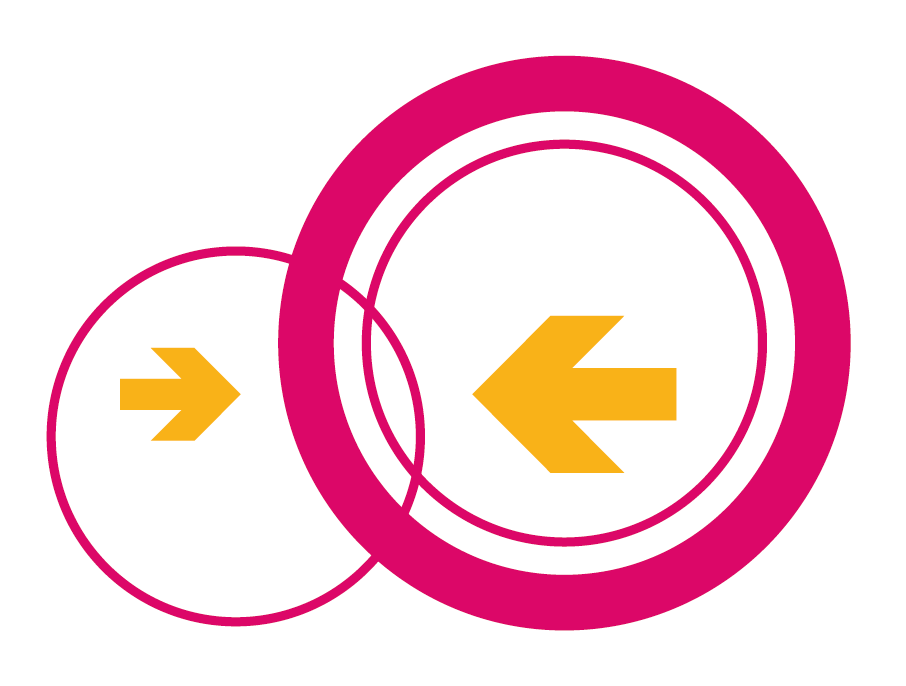
\includegraphics[width=0.1\textwidth]{freifunklogo.png}
\setkomavar{fromname}{Freifunk Aachen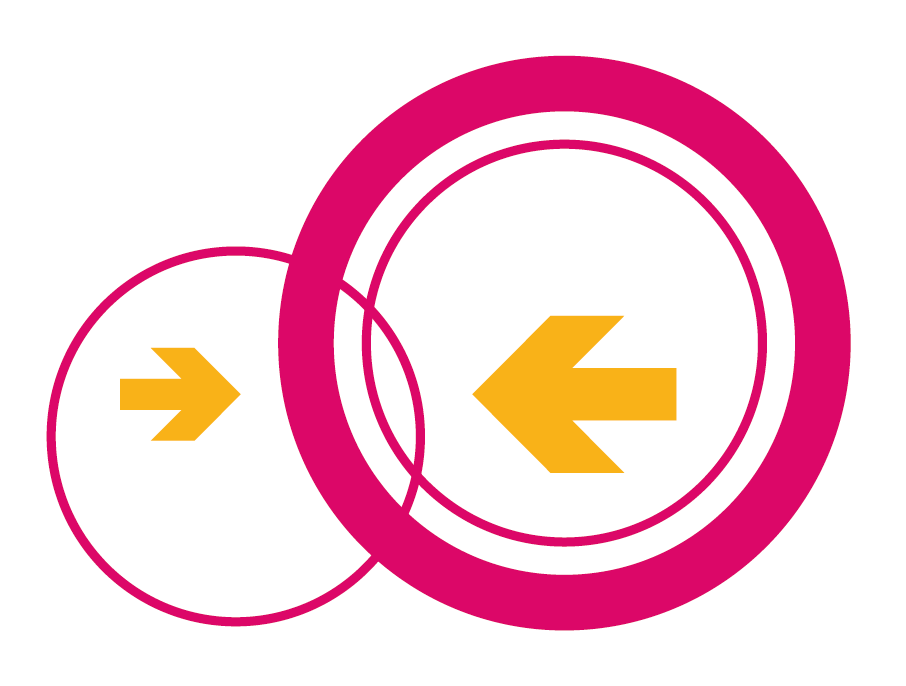
\includegraphics[width=0.1\textwidth]{freifunklogo.png}}
\setkomavar{fromaddress}{Name\\Adresse\\Ort}
\setkomavar{fromphone}[\Mobilefone~]{+49\,(0)\,176\,314\,367\,92}
\setkomavar{fromfax}[\FAX~]{+49\,(0)\,123\,456\,789\,0}
\setkomavar{fromemail}[\Letter~]{@freifunk-aachen.de}
\setkomavar{fromurl}[\faGlobe~]{www.freifunk-aachen.de}
%\setkomafont{fromaddress}{\small\rmfamily\mdseries\slshape\color{myblue}}

%\setkomavar{backaddressseparator}{ - }
\setkomavar{backaddress}{FFAC: Name, Adresse, Ort} % wenn erwünscht kann hier eine andere Backaddress eingetragen werden
\setkomavar{signature}{Name} 
% signature same indention level as rest
\renewcommand*{\raggedsignature}{\raggedright}
%\setkomavar{location}{\raggedleft
%}
% Anlage neu definieren
\renewcommand{\enclname}{Anlagen}
\setkomavar{enclseparator}{: }
%---------------------------------------------------------------------------
% Seitenstil
%pagenumber=footmiddle
\pagestyle{plain}%% keine Header in der Kopfzeile bzw. plain
\pagenumbering{arabic}
%---------------------------------------------------------------------------
%---------------------------------------------------------------------------
\firstfoot{\footnotesize%
\rule[3pt]{\textwidth}{.4pt} \\
\begin{tabular}[t]{l@{}}% 
\usekomavar{fromname}\\
\usekomavar{fromaddress}\\
\end{tabular}%
\hfill
\begin{tabular}[t]{l@{}}%
  \usekomavar[\Mobilefone~]{fromphone}\\
   \usekomavar[\Letter~]{fromemail}\\
\end{tabular}%
\ifkomavarempty{frombank}{}{%
\hfill
\begin{tabular}[t]{l@{}}%
Bankverbindung: \\
\usekomavar{frombank}
\end{tabular}%
}%
}% 
%---------------------------------------------------------------------------
% Bankverbindung
%\setkomavar{frombank}{Kto. 123456789\\
%BLZ 123\,123\,12\\
%Musterbank}
%---------------------------------------------------------------------------
%\setkomavar{yourref}{asd}
%\setkomavar{yourmail}{}
%\setkomavar{myref}{sadf}
%\setkomavar{customer}{}
%\setkomavar{subject}{Rechnungsnummer}
%\setkomavar{invoice}{PS009}
%---------------------------------------------------------------------------
% Datum und Ort werden hier eingetragen
\setkomavar{date}{\today}
\setkomavar{place}{Aachen}
%---------------------------------------------------------------------------

%---------------------------------------------------------------------------
% Hier beginnt der Brief, mit der Anschrift des Empfängers

\begin{letter}
{
Name des Empfängers\\
Straße des Empfängers\\
Ort des Empfängers\\
}
%---------------------------------------------------------------------------
% Der Betreff des Briefes
\setkomavar{subject}{\bf{Betreff...}
}
%---------------------------------------------------------------------------
\opening{Hallo ...,}

hiermit sende ich Dir den angekündigten ... .
Solltest Du noch Fragen oder Anregungen haben, kannst Du Dich gerne wieder bei uns melden.

Anbei habe ich Dir auch einen Mitgliedsantrag für unsere Vereinsförderung hinzugefügt.\\ Wir würden uns freuen, wenn Du uns weiterempfehlst.

\vspace{5pt}


\closing{Viele Grüße,}
%---------------------------------------------------------------------------
%\ps{PS:}
%\cc{}
%---------------------------------------------------------------------------
\end{letter}
%---------------------------------------------------------------------------
\end{document}
%---------------------------------------------------------------------------

